\section{Insert-Furthest-Verfahren} \label{sec:insert-furthest-verfahren}
% Was ist das Insert-Furthest-Verfahren?
    % Nodes werden anhand ihrer Entfernung zur vorherigen Node in den Graphen eingefügt
    % Die am weitest entfernten werden zuerst eingefügt
% Was ist das Insert-Furthest-Verfahren
    % Zu Beginn wird wieder die Erste Node in den Pfad eingefügt, um von ihr ausgehend den restlichen Pfad zu bilden
    % anders als bei Insert First muss bzw. kann hier aber nicht auch die zweite Node eingefügt werden, da diese erst noch ermittelt werden muss
    % Spezifische Auswahl der nächsten einzufügenden Node
    % Die als nächstes eingefügt Node ist immer die, die am weitesten von der zuletzt eingefügten Node entfernt ist 
    % Allerdings muss hier vorher die Bedingung geprüft werden, ob die am weitesten Entfernte node nicht schon im Pfad ist
    % Die am weistesten Entfernte Node wird dann genau wie bei Min Dist ist den bereits existierenden Pfad an der besten verfügbaren Stelle eingefügt
    % Ermittlung der Besten Stelle, in die Node Y eingefügt werden: 
        % Es wird durch alle bereits im Graphen vorhandenen Nodes iteriert
        % Die Node der momentanen Iteration X2, ihr Vorgänger X1
        % Die Distanz berechnet sich aus der Entfernung von X1 zu Y addiert mit der Entfernung von Y zu X2
        % Es wird davon ausgegangen, dass X1 immer definiert, also teil des bereits bestehenden Graphen ist, ist 
        % X2 muss nicht zwangweise definiert sein, kann also auch null sein
        % Ist dies der fall wird für die Distanz zwischen Y und X2 0 angenommen
\subsection{Funktionsweise} \label{sec:insert-furthest-funkt}
Aufbauend auf den Erkenntnissen des Insert-First-Verfahrens können experimentell einige Verbesserungsideen abgeleitet und ihre Auswirkungen auf das Erzeugen eines Graphen betrachtet werden.
Beim Insert-First-Verfahren wurde festgestellt, dass eine große Schwäche des Algorithmus die Reihenfolge der Betrachtung der Knoten sein kann.
Ein möglicher Ansatz, dieser in \vref{sec:inserst-first-erg} beschriebenen Schwäche entgegenzuwirken, ist die Einführung eines Kriteriums zur Betrachtung der Knoten.
Eine mögliche Umsetzung eines solchen Kriteriums ist das Insert-Furthest-Verfahren. 
Hier wird der als nächstes einzufügende Knoten ($k_i$) durch seine Distanz zum Vorgänger ($k_{i-1}$) bestimmt.


% \subsection{Funktionsweise}

Ähnlich dem Insert-First-Verfahren wird auch hier ein Graph mit einer Liste von Knoten und einem zu Beginn leerem Pfad erzeugt.
Auch hier wird wieder der erste Knoten der Liste $k_1$ als initialer Knoten $p_1$ des Pfades $P$ gesetzt.
Der nächste zu betrachtende Knoten ist nun aber nicht $k_2$, sondern wird durch die Distanz zu $k_1$ bestimmt.
Ausgewählt wird der Knoten, der am weitesten von $k_1$, bzw. allgemein am weistesten von $k_{i-1}$, entfernt ist und nicht bereits Teil des Pfads ist.
Dieser Knoten wird nun auf die gleiche Weise wie die Knoten beim Insert-First-Verfahren in den Pfad des Graphen eingefügt; die Stelle mit der geringsten Distanzerhöhung für den Graphen wird gesucht und $k_i$ an dieser Stelle nach dem im \ac{Alg.} \vref{alg:merge-node-into-path} beschriebenen Verfahren eingefügt.\\
Der Gedanke hinter der dieser Veränderung ist der Versuch Knoten mit größerer Vorraussicht als im Insert-First-Verfahren in den Pfad des Graphen einzufügen.
Ziel ist es mit den ersten paar Knoten einen Pfad zu generieren, der einen großen Teil der Fläche überspannt, auf der sich Knoten befinden.
Das kann insofern zu einem besserem Ergebnis führen, dass die ersten Knoten zwar unter einer, relativ zur schlussendlichen Gesamtlänge des Graphen, hohen Distanzerhöhung eingefügt werden, die nachfolgenden Knoten aber durch geringe Umwege des bestehenden Pfads in den Graphen eingebunden werden können.
Auf diese Weise sollen Komplikationen beim Einfügen der letzten Knoten verhindert werden und so suboptimale Graphen wie in \vref{fig:insert-first-bad} umgangen werden.

\begin{algorithm}[H]
    \caption{Insert-Furthest-Algorithmus}
    \label{alg:insert-furthest}
    \begin{algorithmic}[1]
        \Require Graph $G$, Pfad $P$ 
        \Require $G= k_1,k_2,\ldots,k_n$, $n > 2$ 
        % \Require $P=p_1,\cdots,p_m$, $\forall p = k_G$
        \State $p_1 \gets k_1$
        \Comment Setzen des ersten Knoten
        % Find furthest
        \State $i \gets -1$
        \State $d_i \gets -1$

        \For{$a \gets 1$, $a \leq n$, $a \gets a + 1$}
            % Main Loop
            % find Furthest from last
            \State $j_F \gets -1$
            \State $d_F \gets -1$

            \For{$b \gets 2$, $b \leq n$, $b \gets b + 1$}
                \Comment Finde $k_b$ mit der höchsten Distanz zu $p_m$
                \State $d_C \gets \omega$($k_b$, $p_m$)
                \Comment Distanz zwischen $k_b$ und letztem Knoten $p_m$
                \If{$k_b \not \in P$ \textbf{and} ($j_F = -1$ \textbf(or) $d_C > d_F$)}
                    \State $d_F \gets d_C$
                    \State $j_F \gets b$
                \EndIf
            \EndFor

            \State $i_S \gets -1$
            \State $d_S \gets -1$

            \For{$b \gets 2$, $b < m$, $b \gets b + 1$}
                \State $d_C \gets$ \textsc{mergeAt}($P$, $b$, $k_{j_F}$) \textsc{distance}
                \If{$i_S = -1$ \textbf{or} $d_C < d_S$}
                    \State $i_S \gets b$
                    \State $d_S \gets d_C$
                \EndIf
            \EndFor
            \State $P \gets$ \textsc{mergeAt}($P$, $k_{j_F}$, $i_S$)
            \Comment Siehe Alg. \vref{alg:merge-node-into-path}
        \EndFor \\
        \Return new Graph($P$)
    \end{algorithmic}
\end{algorithm}

\subsection{Zeitkomplexität}
Der Insert-Furthest-Algorithmus fügt verglichen mit dem Insert-First-Algorithmus ein Auswahlkriterium hinzu.\\
Dieses Kriterium drückt sich im Pseudocode im \ac{Alg.} \vref{alg:insert-furthest} durch eine zusätzliche Schleife in Zeile vier aus.
Um nun die Zeitkomplexität zu ermitteln, reicht es die Laufzeit dieser Schleife, $n^2$, auf die in \vref{sec:time-comp-first} berechnete zu addieren, wodurch sich 
$$f(n) = \frac{n^2+n}{2}+n^2 -1$$
und dadurch auch hier eine Komplexität von
$$f(n) = O(n^2)$$
ergibt.
Damit skaliert dieser Algorithmus bei sich verändernder Eingabe in etwa genauso wie Insert-First.

\subsection{Ergebnis und Schwächen}
Testet man des Insert-Furthest-Verfahren anhand der Knoten des Beispiels \vref{fig:insert-first-bad} wird sichtbar, dass der Algorithmus tatsächlich in der Lage ist einen besseren Pfad zu generieren als das Insert-First-Verfahren.

\begin{figure}[H]
    \begin{center}
        % \subfloat[$m = 2$\label{subfig:insert-first-BAD-m2}]{%
        % 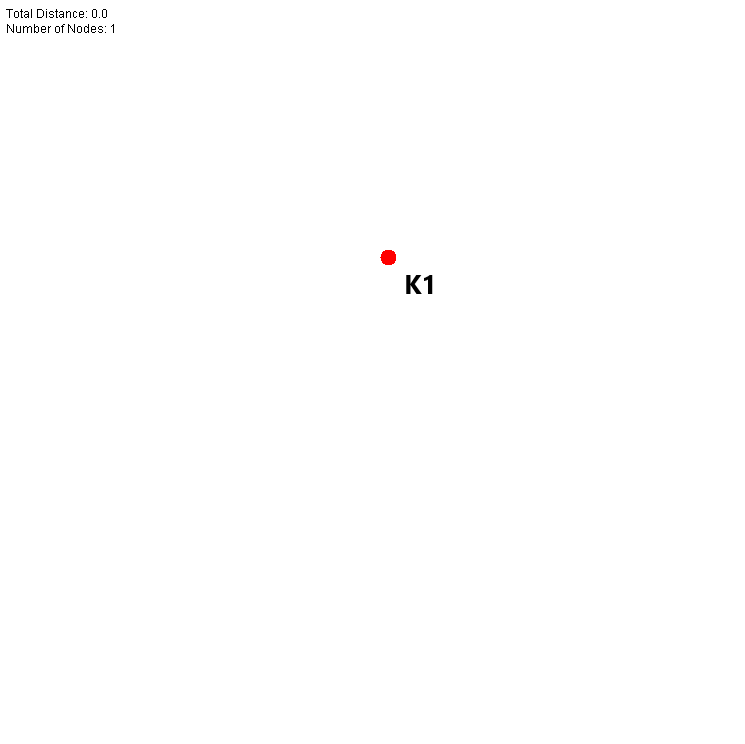
\includegraphics[width=0.35\textwidth]{./Bilder/insertFurthest/insert_furthest_ex_1.PNG}
        % }
        % \hfil
        \subfloat[$m = 2$\label{subfig:insert-furthest-GOOD-m2}]{%
        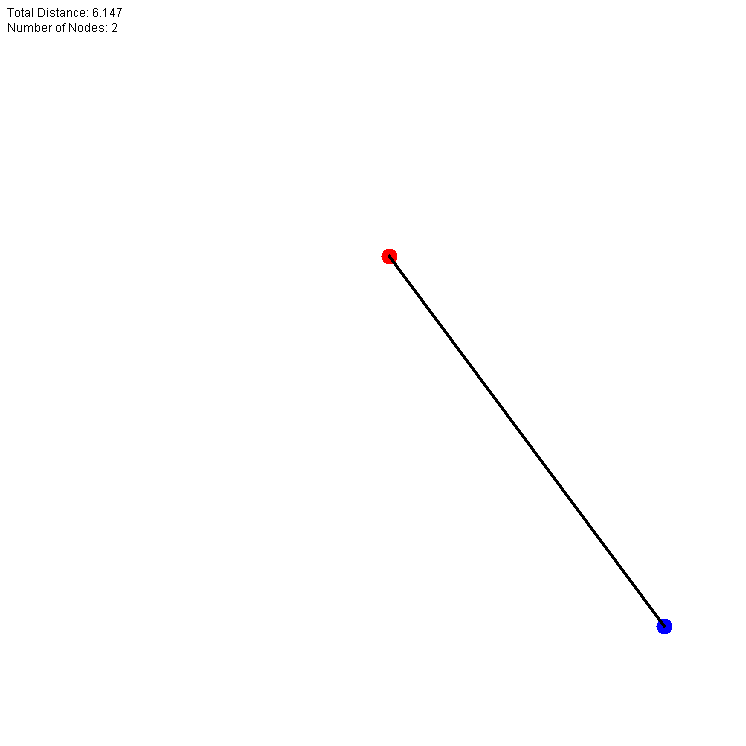
\includegraphics[width=0.35\textwidth]{./Bilder/insertFurthest/insert_furthest_ex_2.PNG}
        }
        % \\
        % \subfloat[$m = 4$\label{subfig:insert-first-BAD-m4}]{%
        % 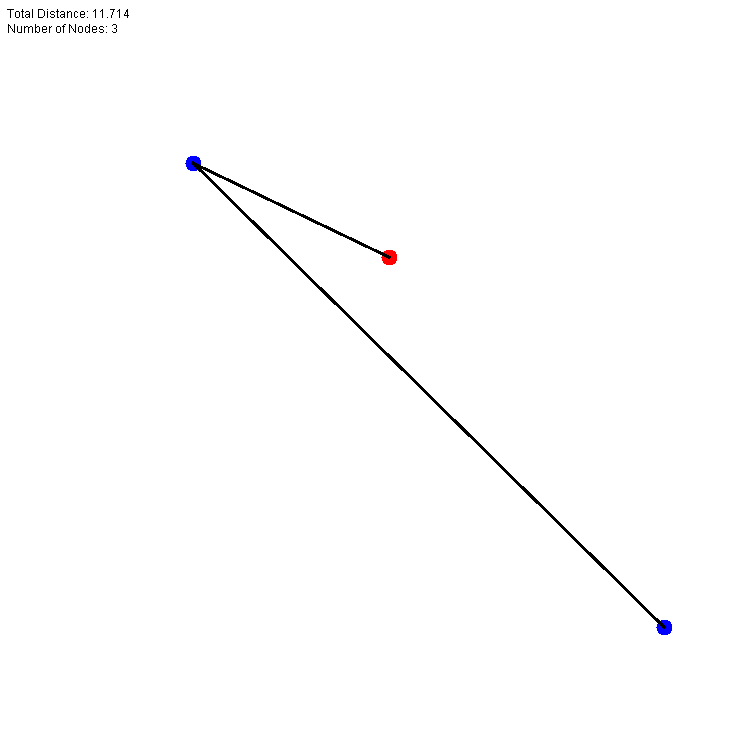
\includegraphics[width=0.35\textwidth]{./Bilder/insertFurthest/insert_furthest_ex_3.PNG}
        % }
        \hfil
        \subfloat[$m = 5$\label{subfig:insert-furthest-GOOD-m5}]{%
        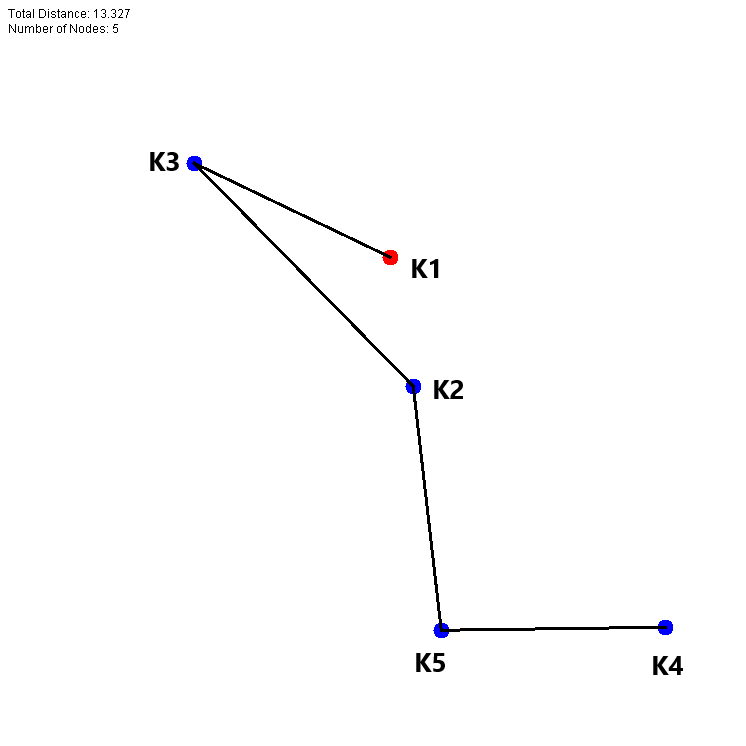
\includegraphics[width=0.35\textwidth]{./Bilder/insertFurthest/insert_furthest_ex_5.PNG}
        }
        \caption{Insert-First führt zu einem gutem Ergebnis}
        \label{fig:insert-furthest-good}
    \end{center}
\end{figure}

% TODO: Alle Schritte/Bilder in den Anhang
In \vref{subfig:insert-furthest-GOOD-m2} ist zu erkennen, dass, anstatt wie in \vref{subfig:insert-first-BAD-m2} $k_2$ als erster Knoten, $k_4$ eingefügt wird.
Dieses Verhalten ist nach der in \vref{sec:insert-furthest-funkt} definierten Funktionsweise zu erwarten, da $k_4$ der Knoten mit der größten Distanz zu $k_1$ ist und daher als erstes in den Pfad des Graphen eingefügt wird.
Nach der Ausführung aller Schritte des Algorithmus erhält man den in \vref{subfig:insert-furthest-GOOD-m5} zu sehenden Graphen.
Dieser hat eine Gesamtdistanz von 13,327 \ac{LE} und ist somit im Vergleich mit dem in \vref{fig:insert-first-bad} durch das Insert-First-Verfahren erzeugten Graph 2,618 \ac{LE} oder 16,41\% kürzer.
\\\\
Ebenso wie das Insert-First-Verfahren kann das Insert-Furthest-Verfahren auch Graphen generieren die in ihrer Gesamtdistanz vom Optimum abweichen. Am folgenden Beispiel wird deutlich, dass auch dieser Algorithmus von ähnlichen Schwächen betroffen ist.
\begin{figure}[H]
    \begin{center}
        % \subfloat[$m = 2$\label{subfig:insert-first-BAD-m2}]{%
        % 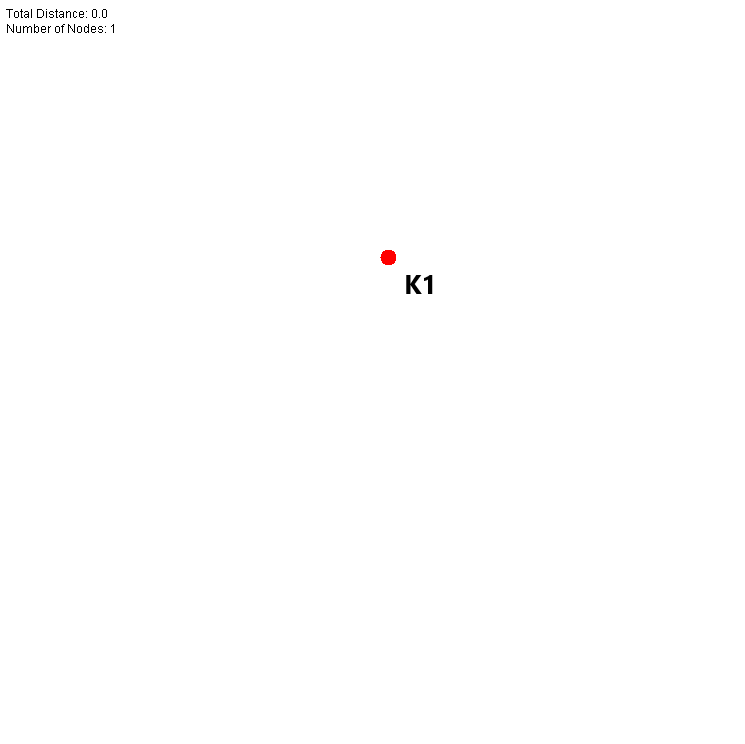
\includegraphics[width=0.35\textwidth]{./Bilder/insertFurthest/insert_furthest_ex_1.PNG}
        % }
        % \hfil
        \subfloat[$m = 4$\label{subfig:insert-furthest-BAD-m2}]{%
        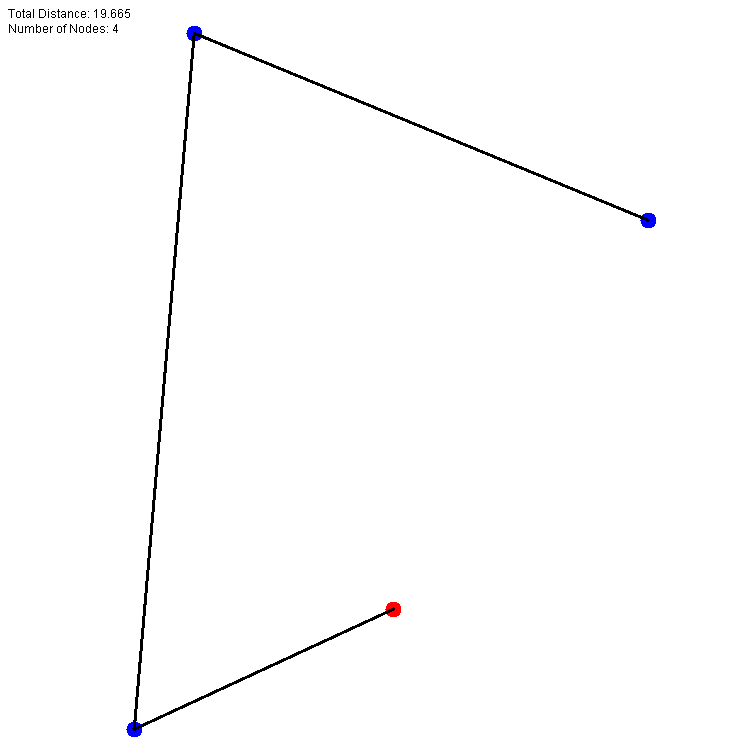
\includegraphics[width=0.35\textwidth]{./Bilder/insertFurthest/insert_furthest_ex_BAD_4.PNG}
        }
        % \\
        % \subfloat[$m = 4$\label{subfig:insert-first-BAD-m4}]{%
        % 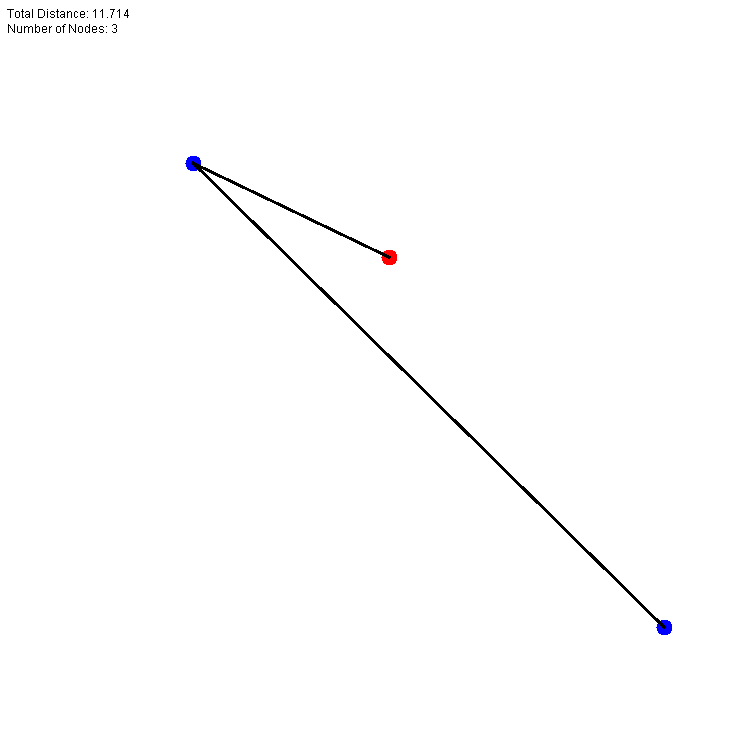
\includegraphics[width=0.35\textwidth]{./Bilder/insertFurthest/insert_furthest_ex_3.PNG}
        % }
        \hfil
        \subfloat[$m = 5$\label{subfig:insert-furthest-BAD-m5}]{%
        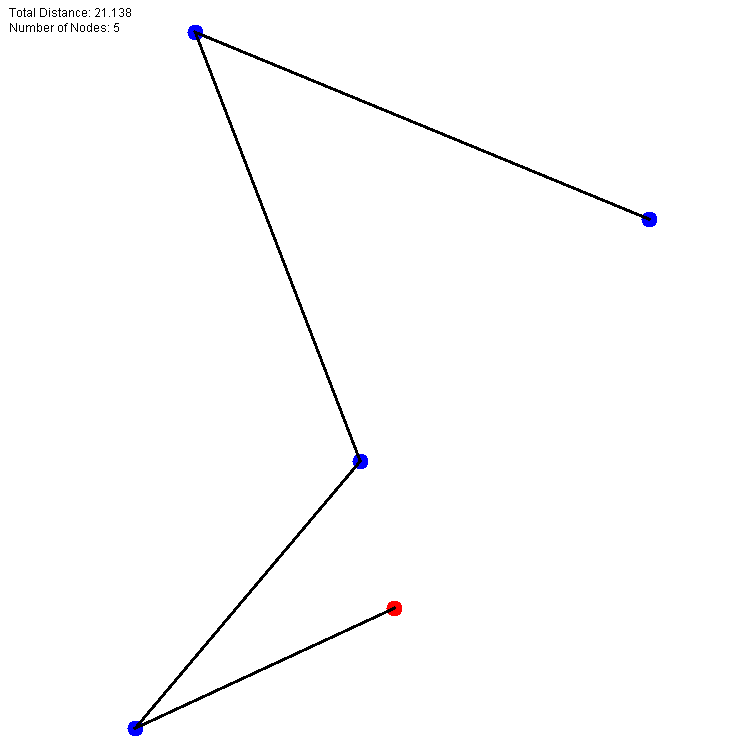
\includegraphics[width=0.35\textwidth]{./Bilder/insertFurthest/insert_furthest_ex_BAD_5.PNG}
        }
        \caption{Insert-First führt zu einem schlechtem Ergebnis}
        \label{fig:insert-furthest-bad}
    \end{center}
\end{figure}
% TODO: Bilder in den Angang
Die der Abbildung \vref{fig:insert-furthest-bad} vorhergehenden Schritte $m=1$ bis $m=3$ sind im Anhang zu finden. 
\\\\
Auch hier lässt sich das Problem der Reihenfolge beobachten, welches in \vref{sec:inserst-first-erg} beschrieben wurde.
Durch das Einfügen des letzten Knotens $k_4$ in den Pfad entsteht ein suboptimaler Graph.
In diesem konkreten Beispiel ist das mit dem menschlichen Auge jedoch nicht sofort ersichtlich.
Vergleicht man aber die Distanzen zwischen den Knoten $k_4$ und $k_1$ (6,129 \ac{LE}) mit den zwischen $k_1$ und $k_2$ (5,019 \ac{LE}) wird schnell ersichtlich, dass eine Verminderung der Distanz durch das Umlegen der Knoten erreicht werden kann.
Verursacht wird diese Abweichung vom Optimum dadurch, dass $k_4$ als letztes in den Graphen eingefügt wird, da der Knoten sich, relativ zu den restlichen Knoten, in der Mitte der Fläche befindet und somit aufgrund seiner geringeren Entfernung vom Algorithmus als betrachtet wird.
Die optimale Route
% \begin{addmargin}[1em]{2em}
$$P = k_1, k_3, k_4, k_2, k_1$$ 
    % \end{addmargin}
 würde es jedoch erfordern, dass $k_4$ früher betrachtet und in den Pfad eingefügt wird.
Der durch den Algorithmus erzeugte Graph hat eine Gesamtlänge von 21,138 \ac{LE}, während durch das Umlegen zum optimalen Graph eine Länge von 20,028 \ac{LE}, also Reduktion der Distanz um 1,11 \ac{LE} oder 5,251\% erreicht werden kann.
\\\\
Das Insert-Furthest-Verfahren verhält sich in einigen Fällen, wie in \vref{fig:insert-furthest-good} gezeigt, besser als das Insert-First-Verfahren, weist aber immer noch eindeutige Schwächen, gerade im Bezug auf die Reihenfolge der Betrachtung der Knoten.
Das Beispiel in \vref{fig:insert-furthest-bad} zeigt deutlich, wie auch hier die Positionierung der Knoten Einfluss auf das Endergebnis hat.